
\documentclass[tikz,border=8pt]{standalone}

\usepackage{fontspec}
\setmainfont{Arial}
\setsansfont{Arial}

\usetikzlibrary{
    arrows.meta,
    positioning,
    fit,
    backgrounds,
    calc
}

\begin{document}

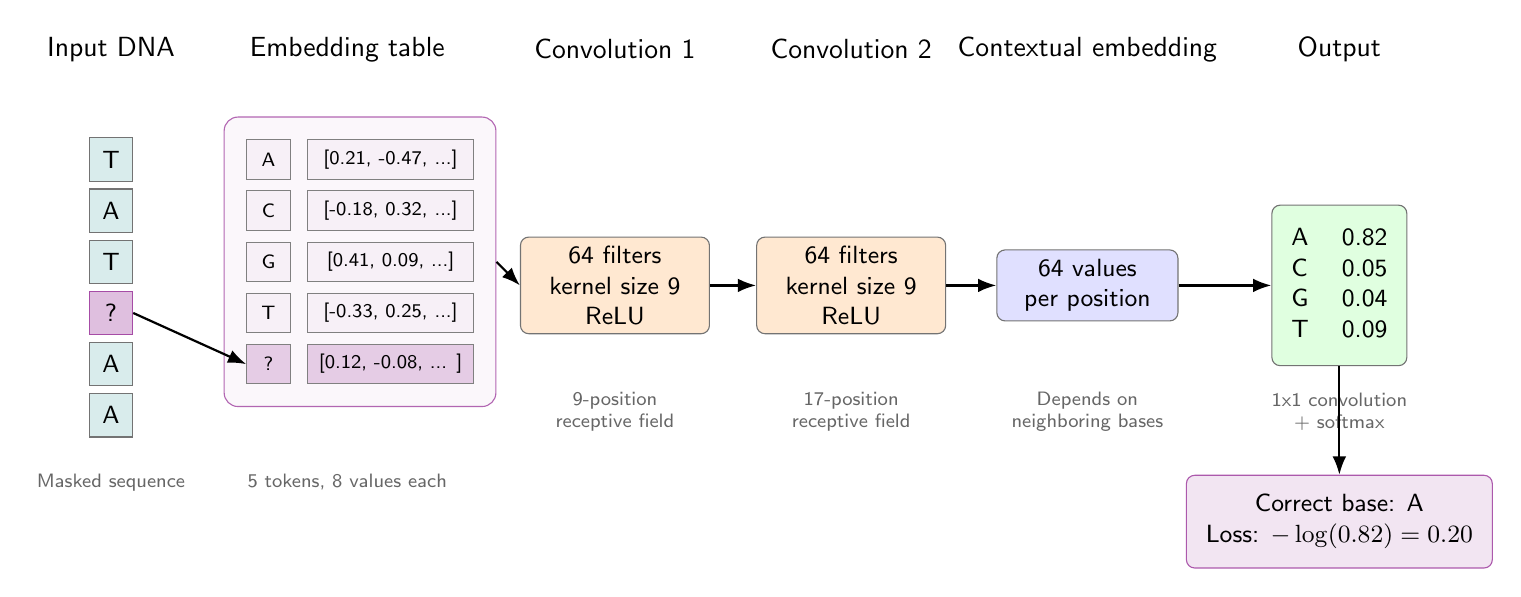
\begin{tikzpicture}[
    >=Latex,
    font=\sffamily,
    arrow/.style={->, thick},
    heading/.style={font=\sffamily, anchor=center},
    base/.style={
        draw=black!55,
        fill=teal!15,
        minimum width=0.55cm,
        minimum height=0.55cm,
        inner sep=0pt,
        font=\sffamily\small
    },
    mask/.style={
        base,
        fill=violet!25,
        draw=violet!70
    },
    layer/.style={
        draw=black!55,
        fill=orange!18,
        rounded corners=3pt,
        minimum width=2.4cm,
        minimum height=0.8cm,
        align=center,
        font=\sffamily\small
    },
    embedding/.style={
        draw=black!55,
        fill=blue!12,
        rounded corners=3pt,
        minimum width=2.3cm,
        minimum height=0.8cm,
        align=center,
        font=\sffamily\small
    }
]

% --------------------------------------------------
% Headings
% --------------------------------------------------

\node[heading] at (0,3.4) {Input DNA};
\node[heading] at (3.0,3.4) {Embedding table};
\node[heading] at (6.4,3.4) {Convolution 1};
\node[heading] at (9.4,3.4) {Convolution 2};
\node[heading] at (12.4,3.4) {Contextual embedding};
\node[heading] at (15.6,3.4) {Output};

% --------------------------------------------------
% Input DNA
% --------------------------------------------------

\foreach \i/\letter in {
    1/T,
    2/A,
    3/T,
    4/?,
    5/A,
    6/A
}{
    \pgfmathsetmacro{\yy}{2.0-(\i-1)*0.65}

    \ifnum\i=4
        \node[mask] (b\i) at (0,\yy) {\letter};
    \else
        \node[base] (b\i) at (0,\yy) {\letter};
    \fi
}

\node[
    font=\sffamily\scriptsize,
    text=black!60
] at (0,-2.1) {Masked sequence};

% --------------------------------------------------
% Embedding lookup table
% 5 tokens x 8 values
% --------------------------------------------------

\foreach \i/\yy/\token/\values in {
    1/2.0/A/{0.21, -0.47, ...},
    2/1.35/C/{-0.18, 0.32, ...},
    3/0.70/G/{0.41, 0.09, ...},
    4/0.05/T/{-0.33, 0.25, ...},
    5/-0.60/?/{0.12, -0.08, ...}
}{
    \ifnum\i=5
        \def\rowfill{violet!20}
    \else
        \def\rowfill{violet!6}
    \fi

    \node[
        draw=black!50,
        fill=\rowfill,
        minimum width=0.55cm,
        minimum height=0.5cm,
        font=\sffamily\scriptsize
    ] (tok\i) at (2.0,\yy) {\token};

    \node[
        draw=black!50,
        fill=\rowfill,
        minimum width=2.1cm,
        minimum height=0.5cm,
        font=\sffamily\scriptsize
    ] (vec\i) at (3.55,\yy) {[\values]};
}

\begin{scope}[on background layer]
\node[
    draw=violet!60,
    fill=violet!3,
    rounded corners=5pt,
    inner sep=8pt,
    fit=(tok1)(vec1)(tok5)(vec5)
] (tablebox) {};
\end{scope}

\draw[arrow] (b4.east) -- (tok5.west);

\node[
    font=\sffamily\scriptsize,
    text=black!60
] at (3.0,-2.1) {5 tokens, 8 values each};

% --------------------------------------------------
% Convolutional layers
% --------------------------------------------------

\node[layer] (conv1) at (6.4,0.4)
    {64 filters\\kernel size 9\\ReLU};

\node[layer] (conv2) at (9.4,0.4)
    {64 filters\\kernel size 9\\ReLU};

\draw[arrow] (tablebox.east) -- (conv1.west);
\draw[arrow] (conv1.east) -- (conv2.west);

\node[
    font=\sffamily\scriptsize,
    text=black!60,
    align=center
] at (6.4,-1.2)
    {9-position\\receptive field};

\node[
    font=\sffamily\scriptsize,
    text=black!60,
    align=center
] at (9.4,-1.2)
    {17-position\\receptive field};

% --------------------------------------------------
% Contextual embedding
% --------------------------------------------------

\node[embedding] (context) at (12.4,0.4)
    {64 values\\per position};

\draw[arrow] (conv2.east) -- (context.west);

\node[
    font=\sffamily\scriptsize,
    text=black!60,
    align=center
] at (12.4,-1.2)
    {Depends on\\neighboring bases};

% --------------------------------------------------
% Output
% --------------------------------------------------

\node[
    draw=black!55,
    fill=green!12,
    rounded corners=3pt,
    inner sep=7pt,
    font=\sffamily\small
] (probs) at (15.6,0.4)
{
    \begin{tabular}{@{}lr@{}}
        A & 0.82 \\
        C & 0.05 \\
        G & 0.04 \\
        T & 0.09
    \end{tabular}
};

\draw[arrow] (context.east) -- (probs.west);

\node[
    font=\sffamily\scriptsize,
    text=black!60,
    align=center
] at (15.6,-1.2)
    {1x1 convolution\\+ softmax};

% --------------------------------------------------
% Loss
% --------------------------------------------------

\node[
    draw=violet!65,
    fill=violet!10,
    rounded corners=3pt,
    inner sep=7pt,
    font=\sffamily\small,
    align=center
] (loss) at (15.6,-2.6)
    {Correct base: A\\
     Loss: $-\log(0.82)=0.20$};

\draw[arrow] (probs.south) -- (loss.north);

\end{tikzpicture}

\end{document}

